\documentclass[twoside]{book}

% Packages required by doxygen
\usepackage{calc}
\usepackage{doxygen}
\usepackage{graphicx}
\usepackage[utf8]{inputenc}
\usepackage{makeidx}
\usepackage{multicol}
\usepackage{multirow}
\usepackage{textcomp}
\usepackage[table]{xcolor}

% Font selection
\usepackage[T1]{fontenc}
\usepackage{mathptmx}
\usepackage[scaled=.90]{helvet}
\usepackage{courier}
\usepackage{amssymb}
\usepackage{sectsty}
\renewcommand{\familydefault}{\sfdefault}
\allsectionsfont{%
  \fontseries{bc}\selectfont%
  \color{darkgray}%
}
\renewcommand{\DoxyLabelFont}{%
  \fontseries{bc}\selectfont%
  \color{darkgray}%
}

% Page & text layout
\usepackage{geometry}
\geometry{%
  a4paper,%
  top=2.5cm,%
  bottom=2.5cm,%
  left=2.5cm,%
  right=2.5cm%
}
\tolerance=750
\hfuzz=15pt
\hbadness=750
\setlength{\emergencystretch}{15pt}
\setlength{\parindent}{0cm}
\setlength{\parskip}{0.2cm}
\makeatletter
\renewcommand{\paragraph}{%
  \@startsection{paragraph}{4}{0ex}{-1.0ex}{1.0ex}{%
    \normalfont\normalsize\bfseries\SS@parafont%
  }%
}
\renewcommand{\subparagraph}{%
  \@startsection{subparagraph}{5}{0ex}{-1.0ex}{1.0ex}{%
    \normalfont\normalsize\bfseries\SS@subparafont%
  }%
}
\makeatother

% Headers & footers
\usepackage{fancyhdr}
\pagestyle{fancyplain}
\fancyhead[LE]{\fancyplain{}{\bfseries\thepage}}
\fancyhead[CE]{\fancyplain{}{}}
\fancyhead[RE]{\fancyplain{}{\bfseries\leftmark}}
\fancyhead[LO]{\fancyplain{}{\bfseries\rightmark}}
\fancyhead[CO]{\fancyplain{}{}}
\fancyhead[RO]{\fancyplain{}{\bfseries\thepage}}
\fancyfoot[LE]{\fancyplain{}{}}
\fancyfoot[CE]{\fancyplain{}{}}
\fancyfoot[RE]{\fancyplain{}{\bfseries\scriptsize Generated on Mon Apr 27 2015 12\-:12\-:07 for My Project by Doxygen }}
\fancyfoot[LO]{\fancyplain{}{\bfseries\scriptsize Generated on Mon Apr 27 2015 12\-:12\-:07 for My Project by Doxygen }}
\fancyfoot[CO]{\fancyplain{}{}}
\fancyfoot[RO]{\fancyplain{}{}}
\renewcommand{\footrulewidth}{0.4pt}
\renewcommand{\chaptermark}[1]{%
  \markboth{#1}{}%
}
\renewcommand{\sectionmark}[1]{%
  \markright{\thesection\ #1}%
}

% Indices & bibliography
\usepackage{natbib}
\usepackage[titles]{tocloft}
\setcounter{tocdepth}{3}
\setcounter{secnumdepth}{5}
\makeindex

% Hyperlinks (required, but should be loaded last)
\usepackage{ifpdf}
\ifpdf
  \usepackage[pdftex,pagebackref=true]{hyperref}
\else
  \usepackage[ps2pdf,pagebackref=true]{hyperref}
\fi
\hypersetup{%
  colorlinks=true,%
  linkcolor=blue,%
  citecolor=blue,%
  unicode%
}

% Custom commands
\newcommand{\clearemptydoublepage}{%
  \newpage{\pagestyle{empty}\cleardoublepage}%
}


%===== C O N T E N T S =====

\begin{document}

% Titlepage & ToC
\hypersetup{pageanchor=false}
\pagenumbering{roman}
\begin{titlepage}
\vspace*{7cm}
\begin{center}%
{\Large My Project }\\
\vspace*{1cm}
{\large Generated by Doxygen 1.8.6}\\
\vspace*{0.5cm}
{\small Mon Apr 27 2015 12:12:07}\\
\end{center}
\end{titlepage}
\clearemptydoublepage
\tableofcontents
\clearemptydoublepage
\pagenumbering{arabic}
\hypersetup{pageanchor=true}

%--- Begin generated contents ---
\chapter{Hierarchical Index}
\section{Class Hierarchy}
This inheritance list is sorted roughly, but not completely, alphabetically\-:\begin{DoxyCompactList}
\item \contentsline{section}{Bounding}{\pageref{classBounding}}{}
\item \contentsline{section}{Camera}{\pageref{classCamera}}{}
\item \contentsline{section}{Events}{\pageref{classEvents}}{}
\item \contentsline{section}{Game\-Asset}{\pageref{classGameAsset}}{}
\begin{DoxyCompactList}
\item \contentsline{section}{Cube\-Asset}{\pageref{classCubeAsset}}{}
\item \contentsline{section}{Diamond\-Asset}{\pageref{classDiamondAsset}}{}
\item \contentsline{section}{Door\-Asset}{\pageref{classDoorAsset}}{}
\end{DoxyCompactList}
\item \contentsline{section}{Game\-Asset\-Manager}{\pageref{classGameAssetManager}}{}
\item \contentsline{section}{Level}{\pageref{classLevel}}{}
\end{DoxyCompactList}

\chapter{Class Index}
\section{Class List}
Here are the classes, structs, unions and interfaces with brief descriptions\-:\begin{DoxyCompactList}
\item\contentsline{section}{\hyperlink{classBounding}{Bounding} }{\pageref{classBounding}}{}
\item\contentsline{section}{\hyperlink{classCamera}{Camera} }{\pageref{classCamera}}{}
\item\contentsline{section}{\hyperlink{classCubeAsset}{Cube\-Asset} }{\pageref{classCubeAsset}}{}
\item\contentsline{section}{\hyperlink{classDiamondAsset}{Diamond\-Asset} }{\pageref{classDiamondAsset}}{}
\item\contentsline{section}{\hyperlink{classDoorAsset}{Door\-Asset} }{\pageref{classDoorAsset}}{}
\item\contentsline{section}{\hyperlink{classEvents}{Events} }{\pageref{classEvents}}{}
\item\contentsline{section}{\hyperlink{classGameAsset}{Game\-Asset} }{\pageref{classGameAsset}}{}
\item\contentsline{section}{\hyperlink{classGameAssetManager}{Game\-Asset\-Manager} }{\pageref{classGameAssetManager}}{}
\item\contentsline{section}{\hyperlink{classLevel}{Level} }{\pageref{classLevel}}{}
\end{DoxyCompactList}

\chapter{Class Documentation}
\hypertarget{classBounding}{\section{Bounding Class Reference}
\label{classBounding}\index{Bounding@{Bounding}}
}


{\ttfamily \#include $<$bounding\-Box.\-h$>$}

\subsection*{Public Member Functions}
\begin{DoxyCompactItemize}
\item 
\hypertarget{classBounding_ac7ed2b50effbd595ded655c77dc5a5bc}{{\bfseries Bounding} (const vec3, float, float, float)}\label{classBounding_ac7ed2b50effbd595ded655c77dc5a5bc}

\item 
float \hyperlink{classBounding_ad1fc6401438da086ae3a74cf5b942d9a}{get\-Width} ()
\item 
float \hyperlink{classBounding_a738f0fd593ae4edd83dc73f26f8ea964}{get\-Height} ()
\item 
float \hyperlink{classBounding_ac5c3654600a9a21d5eae7f6f84ce6137}{get\-Length} ()
\item 
void \hyperlink{classBounding_a276a1ec077a1006cd34a9bd16bbb0fec}{Set\-Centre} (vec3)
\item 
bool \hyperlink{classBounding_a95597f66c6d2bb5b018fdd7eb30b0759}{Collides\-With} (const shared\-\_\-ptr$<$ \hyperlink{classBounding}{Bounding} $>$)
\end{DoxyCompactItemize}
\subsection*{Public Attributes}
\begin{DoxyCompactItemize}
\item 
\hypertarget{classBounding_a5dbd8bfe5d2b3e3e41c2e1e12e53c066}{vec3 {\bfseries pos}}\label{classBounding_a5dbd8bfe5d2b3e3e41c2e1e12e53c066}

\end{DoxyCompactItemize}


\subsection{Detailed Description}
This class follows an algorithm detect if the position and sizes of the assets clash within each other. The class holds multiple methods to return and set information for each of the assets. Being able to access this information makes the algorithm successful. 

\subsection{Member Function Documentation}
\hypertarget{classBounding_a95597f66c6d2bb5b018fdd7eb30b0759}{\index{Bounding@{Bounding}!Collides\-With@{Collides\-With}}
\index{Collides\-With@{Collides\-With}!Bounding@{Bounding}}
\subsubsection[{Collides\-With}]{\setlength{\rightskip}{0pt plus 5cm}bool Bounding\-::\-Collides\-With (
\begin{DoxyParamCaption}
\item[{const shared\-\_\-ptr$<$ {\bf Bounding} $>$}]{b}
\end{DoxyParamCaption}
)}}\label{classBounding_a95597f66c6d2bb5b018fdd7eb30b0759}
Returns true if two objects are colliding -\/ uses an algorithm from commented link \hypertarget{classBounding_a738f0fd593ae4edd83dc73f26f8ea964}{\index{Bounding@{Bounding}!get\-Height@{get\-Height}}
\index{get\-Height@{get\-Height}!Bounding@{Bounding}}
\subsubsection[{get\-Height}]{\setlength{\rightskip}{0pt plus 5cm}float Bounding\-::get\-Height (
\begin{DoxyParamCaption}
{}
\end{DoxyParamCaption}
)}}\label{classBounding_a738f0fd593ae4edd83dc73f26f8ea964}
Returns height \hypertarget{classBounding_ac5c3654600a9a21d5eae7f6f84ce6137}{\index{Bounding@{Bounding}!get\-Length@{get\-Length}}
\index{get\-Length@{get\-Length}!Bounding@{Bounding}}
\subsubsection[{get\-Length}]{\setlength{\rightskip}{0pt plus 5cm}float Bounding\-::get\-Length (
\begin{DoxyParamCaption}
{}
\end{DoxyParamCaption}
)}}\label{classBounding_ac5c3654600a9a21d5eae7f6f84ce6137}
Returns length \hypertarget{classBounding_ad1fc6401438da086ae3a74cf5b942d9a}{\index{Bounding@{Bounding}!get\-Width@{get\-Width}}
\index{get\-Width@{get\-Width}!Bounding@{Bounding}}
\subsubsection[{get\-Width}]{\setlength{\rightskip}{0pt plus 5cm}float Bounding\-::get\-Width (
\begin{DoxyParamCaption}
{}
\end{DoxyParamCaption}
)}}\label{classBounding_ad1fc6401438da086ae3a74cf5b942d9a}
Returns width \hypertarget{classBounding_a276a1ec077a1006cd34a9bd16bbb0fec}{\index{Bounding@{Bounding}!Set\-Centre@{Set\-Centre}}
\index{Set\-Centre@{Set\-Centre}!Bounding@{Bounding}}
\subsubsection[{Set\-Centre}]{\setlength{\rightskip}{0pt plus 5cm}void Bounding\-::\-Set\-Centre (
\begin{DoxyParamCaption}
\item[{vec3}]{v}
\end{DoxyParamCaption}
)}}\label{classBounding_a276a1ec077a1006cd34a9bd16bbb0fec}
Sets a new centre point 

The documentation for this class was generated from the following files\-:\begin{DoxyCompactItemize}
\item 
src/bounding\-Box.\-h\item 
src/bounding\-Box.\-cpp\end{DoxyCompactItemize}

\hypertarget{classCamera}{\section{Camera Class Reference}
\label{classCamera}\index{Camera@{Camera}}
}


{\ttfamily \#include $<$camera.\-h$>$}

\subsection*{Public Member Functions}
\begin{DoxyCompactItemize}
\item 
glm\-::mat4 \hyperlink{classCamera_adf09522521723786b9f405c99d6594c7}{get\-Projection\-Matrix} ()
\item 
glm\-::mat4 \hyperlink{classCamera_a5569ca5967e01d3344fbf6aba36d9820}{get\-View\-Matrix} ()
\item 
void \hyperlink{classCamera_a3be70f5bbcb806eb902a82dbb17e6bc3}{move\-Forward} (float dt)
\item 
void \hyperlink{classCamera_a3aa8d25c1e36af10fac1f749a1bb420e}{move\-Backward} (float dt)
\item 
void \hyperlink{classCamera_a4ec8b9654ae4fa6274920891321899b7}{mouse\-Movement} (float dt)
\item 
void \hyperlink{classCamera_a4d12c50b0d5306860f4e1493374e6fc9}{jumping} (float dt)
\item 
bool \hyperlink{classCamera_a08f5ef4dc4d503d539635a6bd80bd095}{currently\-Falling} ()
\item 
void \hyperlink{classCamera_a6889ceabc0a2d71fa0eb83268d628b94}{set\-Jump} (bool j)
\item 
void \hyperlink{classCamera_aea3ceffb4ff1a209995820e20910f21f}{set\-Gravity} (bool g)
\item 
void \hyperlink{classCamera_a6165c2b248c2675194dd6505b0099cf2}{reset\-Pos} ()
\item 
void \hyperlink{classCamera_ace63ab83e5ec884fee9d2acad85dde03}{falling} (float d\-Time)
\item 
glm\-::vec3 \hyperlink{classCamera_ab779e5b58cc0cddcd0738a13d82aa523}{Get\-Pos} ()
\item 
void \hyperlink{classCamera_a0edb621b581804dcd1ed129082045f7e}{camera\-Controls} (S\-D\-L\-\_\-\-Window $\ast$window)
\end{DoxyCompactItemize}


\subsection{Detailed Description}
This class uses the most mathmatics within our program, following the direction $\ast$ time $\ast$ speed algorithm to move the camera around the game world. 

\subsection{Member Function Documentation}
\hypertarget{classCamera_a0edb621b581804dcd1ed129082045f7e}{\index{Camera@{Camera}!camera\-Controls@{camera\-Controls}}
\index{camera\-Controls@{camera\-Controls}!Camera@{Camera}}
\subsubsection[{camera\-Controls}]{\setlength{\rightskip}{0pt plus 5cm}void Camera\-::camera\-Controls (
\begin{DoxyParamCaption}
\item[{S\-D\-L\-\_\-\-Window $\ast$}]{window}
\end{DoxyParamCaption}
)}}\label{classCamera_a0edb621b581804dcd1ed129082045f7e}
Several things occur here, but its main purpose is to update the camera position and direction as well as manage variables like jumping and gravity \hypertarget{classCamera_a08f5ef4dc4d503d539635a6bd80bd095}{\index{Camera@{Camera}!currently\-Falling@{currently\-Falling}}
\index{currently\-Falling@{currently\-Falling}!Camera@{Camera}}
\subsubsection[{currently\-Falling}]{\setlength{\rightskip}{0pt plus 5cm}bool Camera\-::currently\-Falling (
\begin{DoxyParamCaption}
{}
\end{DoxyParamCaption}
)}}\label{classCamera_a08f5ef4dc4d503d539635a6bd80bd095}
Returns the status of gravity \hypertarget{classCamera_ace63ab83e5ec884fee9d2acad85dde03}{\index{Camera@{Camera}!falling@{falling}}
\index{falling@{falling}!Camera@{Camera}}
\subsubsection[{falling}]{\setlength{\rightskip}{0pt plus 5cm}void Camera\-::falling (
\begin{DoxyParamCaption}
\item[{float}]{d\-Time}
\end{DoxyParamCaption}
)}}\label{classCamera_ace63ab83e5ec884fee9d2acad85dde03}
Y decrements by d\-Time $\ast$ speed \hypertarget{classCamera_ab779e5b58cc0cddcd0738a13d82aa523}{\index{Camera@{Camera}!Get\-Pos@{Get\-Pos}}
\index{Get\-Pos@{Get\-Pos}!Camera@{Camera}}
\subsubsection[{Get\-Pos}]{\setlength{\rightskip}{0pt plus 5cm}glm\-::vec3 Camera\-::\-Get\-Pos (
\begin{DoxyParamCaption}
{}
\end{DoxyParamCaption}
)}}\label{classCamera_ab779e5b58cc0cddcd0738a13d82aa523}
Returns the cameras current position \hypertarget{classCamera_adf09522521723786b9f405c99d6594c7}{\index{Camera@{Camera}!get\-Projection\-Matrix@{get\-Projection\-Matrix}}
\index{get\-Projection\-Matrix@{get\-Projection\-Matrix}!Camera@{Camera}}
\subsubsection[{get\-Projection\-Matrix}]{\setlength{\rightskip}{0pt plus 5cm}glm\-::mat4 Camera\-::get\-Projection\-Matrix (
\begin{DoxyParamCaption}
{}
\end{DoxyParamCaption}
)}}\label{classCamera_adf09522521723786b9f405c99d6594c7}
Need for translating cubes from model to world space \hypertarget{classCamera_a5569ca5967e01d3344fbf6aba36d9820}{\index{Camera@{Camera}!get\-View\-Matrix@{get\-View\-Matrix}}
\index{get\-View\-Matrix@{get\-View\-Matrix}!Camera@{Camera}}
\subsubsection[{get\-View\-Matrix}]{\setlength{\rightskip}{0pt plus 5cm}glm\-::mat4 Camera\-::get\-View\-Matrix (
\begin{DoxyParamCaption}
{}
\end{DoxyParamCaption}
)}}\label{classCamera_a5569ca5967e01d3344fbf6aba36d9820}
Need for translating cubes from model to world space \hypertarget{classCamera_a4d12c50b0d5306860f4e1493374e6fc9}{\index{Camera@{Camera}!jumping@{jumping}}
\index{jumping@{jumping}!Camera@{Camera}}
\subsubsection[{jumping}]{\setlength{\rightskip}{0pt plus 5cm}void Camera\-::jumping (
\begin{DoxyParamCaption}
\item[{float}]{d\-Time}
\end{DoxyParamCaption}
)}}\label{classCamera_a4d12c50b0d5306860f4e1493374e6fc9}
If jumping is true then Y is incremented by d\-Time $\ast$ speed, but if it exceeds Y + 2 then stop jumping \hypertarget{classCamera_a4ec8b9654ae4fa6274920891321899b7}{\index{Camera@{Camera}!mouse\-Movement@{mouse\-Movement}}
\index{mouse\-Movement@{mouse\-Movement}!Camera@{Camera}}
\subsubsection[{mouse\-Movement}]{\setlength{\rightskip}{0pt plus 5cm}void Camera\-::mouse\-Movement (
\begin{DoxyParamCaption}
\item[{float}]{d\-Time}
\end{DoxyParamCaption}
)}}\label{classCamera_a4ec8b9654ae4fa6274920891321899b7}
Uses the mouses position to determine where the camera is looking \hypertarget{classCamera_a3aa8d25c1e36af10fac1f749a1bb420e}{\index{Camera@{Camera}!move\-Backward@{move\-Backward}}
\index{move\-Backward@{move\-Backward}!Camera@{Camera}}
\subsubsection[{move\-Backward}]{\setlength{\rightskip}{0pt plus 5cm}void Camera\-::move\-Backward (
\begin{DoxyParamCaption}
\item[{float}]{d\-Time}
\end{DoxyParamCaption}
)}}\label{classCamera_a3aa8d25c1e36af10fac1f749a1bb420e}
If S is pressed then camera moves forward, based on where the camera is facing. Y is moved by 0.\-0f (So it doesn't move) \hypertarget{classCamera_a3be70f5bbcb806eb902a82dbb17e6bc3}{\index{Camera@{Camera}!move\-Forward@{move\-Forward}}
\index{move\-Forward@{move\-Forward}!Camera@{Camera}}
\subsubsection[{move\-Forward}]{\setlength{\rightskip}{0pt plus 5cm}void Camera\-::move\-Forward (
\begin{DoxyParamCaption}
\item[{float}]{d\-Time}
\end{DoxyParamCaption}
)}}\label{classCamera_a3be70f5bbcb806eb902a82dbb17e6bc3}
If W is pressed then camera moves forward, based on where the camera is facing. Y is moved by 0.\-0f (So it doesn't move) \hypertarget{classCamera_a6165c2b248c2675194dd6505b0099cf2}{\index{Camera@{Camera}!reset\-Pos@{reset\-Pos}}
\index{reset\-Pos@{reset\-Pos}!Camera@{Camera}}
\subsubsection[{reset\-Pos}]{\setlength{\rightskip}{0pt plus 5cm}void Camera\-::reset\-Pos (
\begin{DoxyParamCaption}
{}
\end{DoxyParamCaption}
)}}\label{classCamera_a6165c2b248c2675194dd6505b0099cf2}
Resets the position of the gravity \hypertarget{classCamera_aea3ceffb4ff1a209995820e20910f21f}{\index{Camera@{Camera}!set\-Gravity@{set\-Gravity}}
\index{set\-Gravity@{set\-Gravity}!Camera@{Camera}}
\subsubsection[{set\-Gravity}]{\setlength{\rightskip}{0pt plus 5cm}void Camera\-::set\-Gravity (
\begin{DoxyParamCaption}
\item[{bool}]{g}
\end{DoxyParamCaption}
)}}\label{classCamera_aea3ceffb4ff1a209995820e20910f21f}
Sets gravity to true or false \hypertarget{classCamera_a6889ceabc0a2d71fa0eb83268d628b94}{\index{Camera@{Camera}!set\-Jump@{set\-Jump}}
\index{set\-Jump@{set\-Jump}!Camera@{Camera}}
\subsubsection[{set\-Jump}]{\setlength{\rightskip}{0pt plus 5cm}void Camera\-::set\-Jump (
\begin{DoxyParamCaption}
\item[{bool}]{j}
\end{DoxyParamCaption}
)}}\label{classCamera_a6889ceabc0a2d71fa0eb83268d628b94}
Sets jump to true or false 

The documentation for this class was generated from the following files\-:\begin{DoxyCompactItemize}
\item 
src/camera.\-h\item 
src/camera.\-cpp\end{DoxyCompactItemize}

\hypertarget{classCubeAsset}{\section{Cube\-Asset Class Reference}
\label{classCubeAsset}\index{Cube\-Asset@{Cube\-Asset}}
}


{\ttfamily \#include $<$Cube\-Asset.\-h$>$}

Inheritance diagram for Cube\-Asset\-:\begin{figure}[H]
\begin{center}
\leavevmode
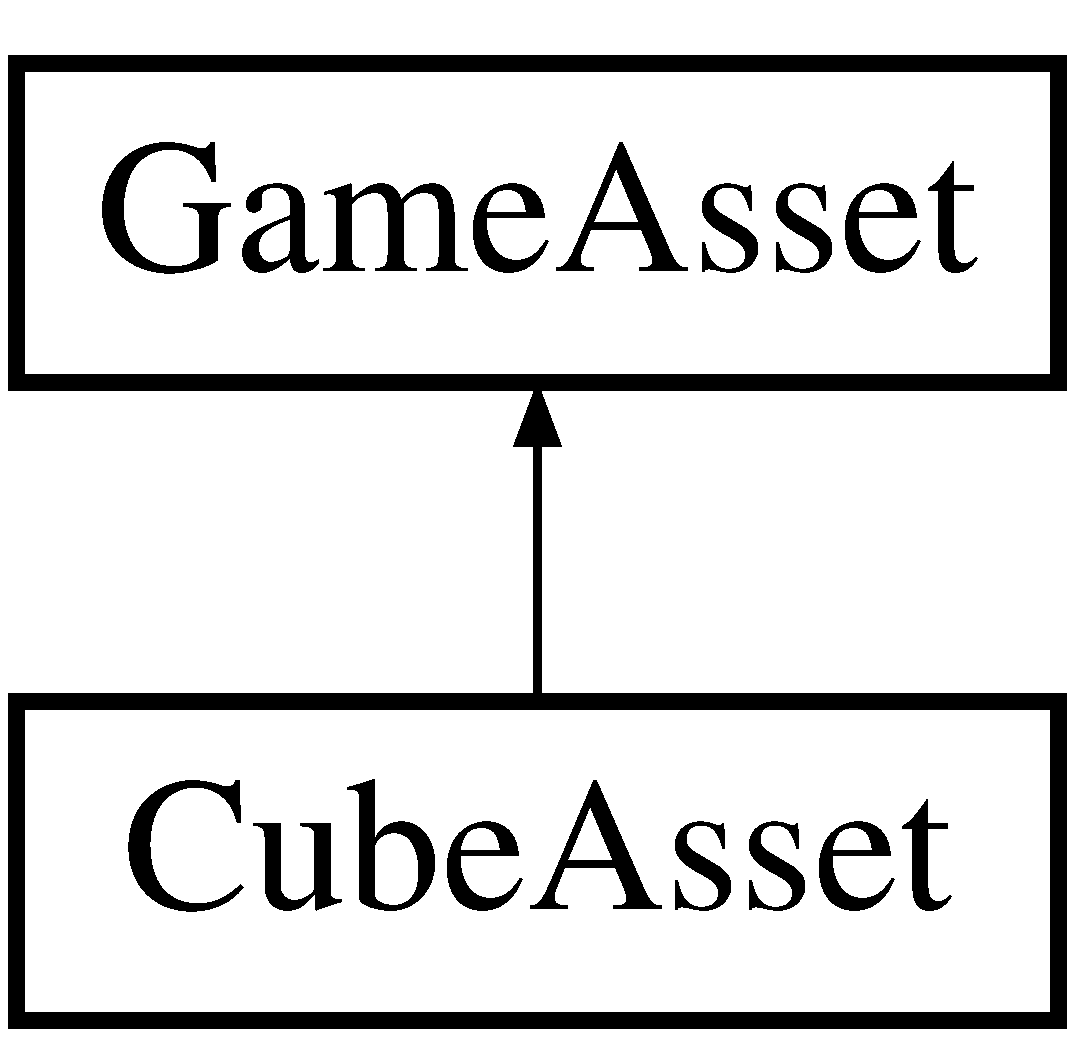
\includegraphics[height=2.000000cm]{classCubeAsset}
\end{center}
\end{figure}
\subsection*{Public Member Functions}
\begin{DoxyCompactItemize}
\item 
\hypertarget{classCubeAsset_a9eb4b26fb2bab2c821cf8566b44dabb8}{{\bfseries Cube\-Asset} (int num)}\label{classCubeAsset_a9eb4b26fb2bab2c821cf8566b44dabb8}

\item 
virtual void \hyperlink{classCubeAsset_a7396ae86ceb988edd1fb9b21903cdaa4}{Draw} (G\-Luint program\-I\-D, \hyperlink{classCamera}{Camera} player)
\item 
virtual void \hyperlink{classCubeAsset_a4a934009bd945ac659b2658400af505d}{New\-Position} (vec3)
\item 
virtual bool \hyperlink{classCubeAsset_a4ee70be683d43e15041ee1cfb44cc0f4}{Collides} (const shared\-\_\-ptr$<$ \hyperlink{classBounding}{Bounding} $>$ b)
\item 
virtual vec3 \hyperlink{classCubeAsset_a82c603031c83dce2921aa2611e5385c7}{Get\-Pos} ()
\item 
virtual std\-::shared\-\_\-ptr$<$ \hyperlink{classBounding}{Bounding} $>$ \hyperlink{classCubeAsset_a8de727c3264ddba5167b2cf453258eb1}{Get\-Box} ()
\end{DoxyCompactItemize}


\subsection{Detailed Description}
The fire \hyperlink{classGameAsset}{Game\-Asset} which reads in an int to determine its x and y factor, meaning that this asset will vary in size. It also uses this int to create a bounding box of a certain size. This change allowed us to make the levels more interesting, and use the varying cube sizes to add further challenge to the game. 

\subsection{Member Function Documentation}
\hypertarget{classCubeAsset_a4ee70be683d43e15041ee1cfb44cc0f4}{\index{Cube\-Asset@{Cube\-Asset}!Collides@{Collides}}
\index{Collides@{Collides}!CubeAsset@{Cube\-Asset}}
\subsubsection[{Collides}]{\setlength{\rightskip}{0pt plus 5cm}bool Cube\-Asset\-::\-Collides (
\begin{DoxyParamCaption}
\item[{const shared\-\_\-ptr$<$ {\bf Bounding} $>$}]{b}
\end{DoxyParamCaption}
)\hspace{0.3cm}{\ttfamily [virtual]}}}\label{classCubeAsset_a4ee70be683d43e15041ee1cfb44cc0f4}
Returns true if two things are colliding 

Implements \hyperlink{classGameAsset}{Game\-Asset}.

\hypertarget{classCubeAsset_a7396ae86ceb988edd1fb9b21903cdaa4}{\index{Cube\-Asset@{Cube\-Asset}!Draw@{Draw}}
\index{Draw@{Draw}!CubeAsset@{Cube\-Asset}}
\subsubsection[{Draw}]{\setlength{\rightskip}{0pt plus 5cm}void Cube\-Asset\-::\-Draw (
\begin{DoxyParamCaption}
\item[{G\-Luint}]{program\-I\-D, }
\item[{{\bf Camera}}]{player}
\end{DoxyParamCaption}
)\hspace{0.3cm}{\ttfamily [virtual]}}}\label{classCubeAsset_a7396ae86ceb988edd1fb9b21903cdaa4}
Draws the cubes onto the screen 

Implements \hyperlink{classGameAsset}{Game\-Asset}.

\hypertarget{classCubeAsset_a8de727c3264ddba5167b2cf453258eb1}{\index{Cube\-Asset@{Cube\-Asset}!Get\-Box@{Get\-Box}}
\index{Get\-Box@{Get\-Box}!CubeAsset@{Cube\-Asset}}
\subsubsection[{Get\-Box}]{\setlength{\rightskip}{0pt plus 5cm}std\-::shared\-\_\-ptr$<$ {\bf Bounding} $>$ Cube\-Asset\-::\-Get\-Box (
\begin{DoxyParamCaption}
{}
\end{DoxyParamCaption}
)\hspace{0.3cm}{\ttfamily [virtual]}}}\label{classCubeAsset_a8de727c3264ddba5167b2cf453258eb1}
Obtains the assets B\-B 

Implements \hyperlink{classGameAsset}{Game\-Asset}.

\hypertarget{classCubeAsset_a82c603031c83dce2921aa2611e5385c7}{\index{Cube\-Asset@{Cube\-Asset}!Get\-Pos@{Get\-Pos}}
\index{Get\-Pos@{Get\-Pos}!CubeAsset@{Cube\-Asset}}
\subsubsection[{Get\-Pos}]{\setlength{\rightskip}{0pt plus 5cm}vec3 Cube\-Asset\-::\-Get\-Pos (
\begin{DoxyParamCaption}
{}
\end{DoxyParamCaption}
)\hspace{0.3cm}{\ttfamily [virtual]}}}\label{classCubeAsset_a82c603031c83dce2921aa2611e5385c7}
Returns the cubes position 

Implements \hyperlink{classGameAsset}{Game\-Asset}.

\hypertarget{classCubeAsset_a4a934009bd945ac659b2658400af505d}{\index{Cube\-Asset@{Cube\-Asset}!New\-Position@{New\-Position}}
\index{New\-Position@{New\-Position}!CubeAsset@{Cube\-Asset}}
\subsubsection[{New\-Position}]{\setlength{\rightskip}{0pt plus 5cm}void Cube\-Asset\-::\-New\-Position (
\begin{DoxyParamCaption}
\item[{vec3}]{pos}
\end{DoxyParamCaption}
)\hspace{0.3cm}{\ttfamily [virtual]}}}\label{classCubeAsset_a4a934009bd945ac659b2658400af505d}
Sets a new translating position, as well as a switch to handle B\-B issue 

The documentation for this class was generated from the following files\-:\begin{DoxyCompactItemize}
\item 
src/Cube\-Asset.\-h\item 
src/Cube\-Asset.\-cpp\end{DoxyCompactItemize}

\hypertarget{classDiamondAsset}{\section{Diamond\-Asset Class Reference}
\label{classDiamondAsset}\index{Diamond\-Asset@{Diamond\-Asset}}
}


{\ttfamily \#include $<$diamond\-Asset.\-h$>$}

Inheritance diagram for Diamond\-Asset\-:\begin{figure}[H]
\begin{center}
\leavevmode
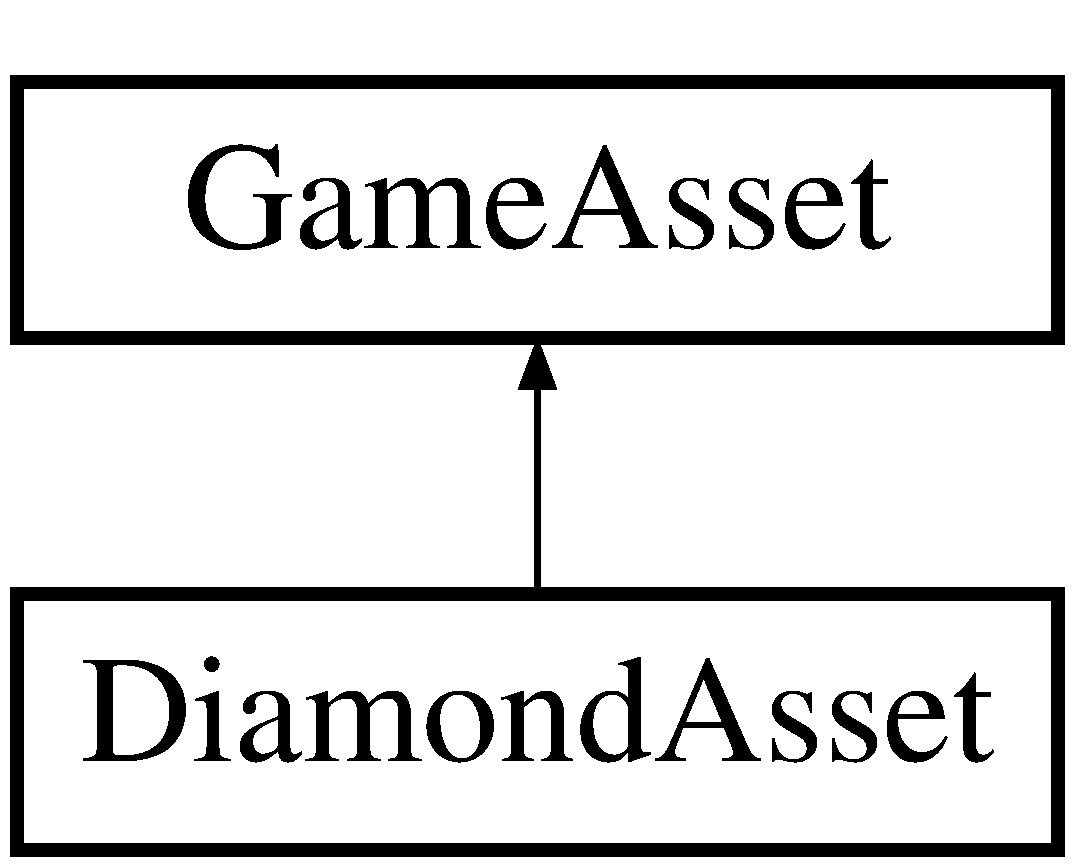
\includegraphics[height=2.000000cm]{classDiamondAsset}
\end{center}
\end{figure}
\subsection*{Public Member Functions}
\begin{DoxyCompactItemize}
\item 
virtual void \hyperlink{classDiamondAsset_a802d11c439859b048533a94fbe662e96}{Draw} (G\-Luint program\-I\-D, \hyperlink{classCamera}{Camera} player)
\item 
virtual void \hyperlink{classDiamondAsset_a266fe301cfa7fc82195d85d29901a6b8}{New\-Position} (vec3)
\item 
virtual bool \hyperlink{classDiamondAsset_af6f6a31e3f6c52e1980f270fd153f0ae}{Collides} (const shared\-\_\-ptr$<$ \hyperlink{classBounding}{Bounding} $>$ b)
\item 
virtual vec3 \hyperlink{classDiamondAsset_aa387857fb5c62227b671500b28cee4df}{Get\-Pos} ()
\item 
virtual std\-::shared\-\_\-ptr$<$ \hyperlink{classBounding}{Bounding} $>$ \hyperlink{classDiamondAsset_acb927e5213c69cf7042bdb80b984b033}{Get\-Box} ()
\end{DoxyCompactItemize}


\subsection{Detailed Description}
The design for this \hyperlink{classGameAsset}{Game\-Asset} was to turn the cube 90\% and bring the points together, so it becomes a diamond. It follows the same element buffer as the cube, so you'll notice a lot of similarities between this and the \hyperlink{classCubeAsset}{Cube\-Asset} but the points had to be very different. 

\subsection{Member Function Documentation}
\hypertarget{classDiamondAsset_af6f6a31e3f6c52e1980f270fd153f0ae}{\index{Diamond\-Asset@{Diamond\-Asset}!Collides@{Collides}}
\index{Collides@{Collides}!DiamondAsset@{Diamond\-Asset}}
\subsubsection[{Collides}]{\setlength{\rightskip}{0pt plus 5cm}bool Diamond\-Asset\-::\-Collides (
\begin{DoxyParamCaption}
\item[{const shared\-\_\-ptr$<$ {\bf Bounding} $>$}]{b}
\end{DoxyParamCaption}
)\hspace{0.3cm}{\ttfamily [virtual]}}}\label{classDiamondAsset_af6f6a31e3f6c52e1980f270fd153f0ae}
Returns true if two things are colliding 

Implements \hyperlink{classGameAsset}{Game\-Asset}.

\hypertarget{classDiamondAsset_a802d11c439859b048533a94fbe662e96}{\index{Diamond\-Asset@{Diamond\-Asset}!Draw@{Draw}}
\index{Draw@{Draw}!DiamondAsset@{Diamond\-Asset}}
\subsubsection[{Draw}]{\setlength{\rightskip}{0pt plus 5cm}void Diamond\-Asset\-::\-Draw (
\begin{DoxyParamCaption}
\item[{G\-Luint}]{program\-I\-D, }
\item[{{\bf Camera}}]{player}
\end{DoxyParamCaption}
)\hspace{0.3cm}{\ttfamily [virtual]}}}\label{classDiamondAsset_a802d11c439859b048533a94fbe662e96}
Draws the diamonds onto the screen 

Implements \hyperlink{classGameAsset}{Game\-Asset}.

\hypertarget{classDiamondAsset_acb927e5213c69cf7042bdb80b984b033}{\index{Diamond\-Asset@{Diamond\-Asset}!Get\-Box@{Get\-Box}}
\index{Get\-Box@{Get\-Box}!DiamondAsset@{Diamond\-Asset}}
\subsubsection[{Get\-Box}]{\setlength{\rightskip}{0pt plus 5cm}std\-::shared\-\_\-ptr$<$ {\bf Bounding} $>$ Diamond\-Asset\-::\-Get\-Box (
\begin{DoxyParamCaption}
{}
\end{DoxyParamCaption}
)\hspace{0.3cm}{\ttfamily [virtual]}}}\label{classDiamondAsset_acb927e5213c69cf7042bdb80b984b033}
Obtains the assets B\-B 

Implements \hyperlink{classGameAsset}{Game\-Asset}.

\hypertarget{classDiamondAsset_aa387857fb5c62227b671500b28cee4df}{\index{Diamond\-Asset@{Diamond\-Asset}!Get\-Pos@{Get\-Pos}}
\index{Get\-Pos@{Get\-Pos}!DiamondAsset@{Diamond\-Asset}}
\subsubsection[{Get\-Pos}]{\setlength{\rightskip}{0pt plus 5cm}vec3 Diamond\-Asset\-::\-Get\-Pos (
\begin{DoxyParamCaption}
{}
\end{DoxyParamCaption}
)\hspace{0.3cm}{\ttfamily [virtual]}}}\label{classDiamondAsset_aa387857fb5c62227b671500b28cee4df}
Returns the diamonds position 

Implements \hyperlink{classGameAsset}{Game\-Asset}.

\hypertarget{classDiamondAsset_a266fe301cfa7fc82195d85d29901a6b8}{\index{Diamond\-Asset@{Diamond\-Asset}!New\-Position@{New\-Position}}
\index{New\-Position@{New\-Position}!DiamondAsset@{Diamond\-Asset}}
\subsubsection[{New\-Position}]{\setlength{\rightskip}{0pt plus 5cm}void Diamond\-Asset\-::\-New\-Position (
\begin{DoxyParamCaption}
\item[{vec3}]{pos}
\end{DoxyParamCaption}
)\hspace{0.3cm}{\ttfamily [virtual]}}}\label{classDiamondAsset_a266fe301cfa7fc82195d85d29901a6b8}
Sets a new translating position 

The documentation for this class was generated from the following files\-:\begin{DoxyCompactItemize}
\item 
src/diamond\-Asset.\-h\item 
src/diamond\-Asset.\-cpp\end{DoxyCompactItemize}

\hypertarget{classDoorAsset}{\section{Door\-Asset Class Reference}
\label{classDoorAsset}\index{Door\-Asset@{Door\-Asset}}
}


{\ttfamily \#include $<$Door\-Asset.\-h$>$}

Inheritance diagram for Door\-Asset\-:\begin{figure}[H]
\begin{center}
\leavevmode
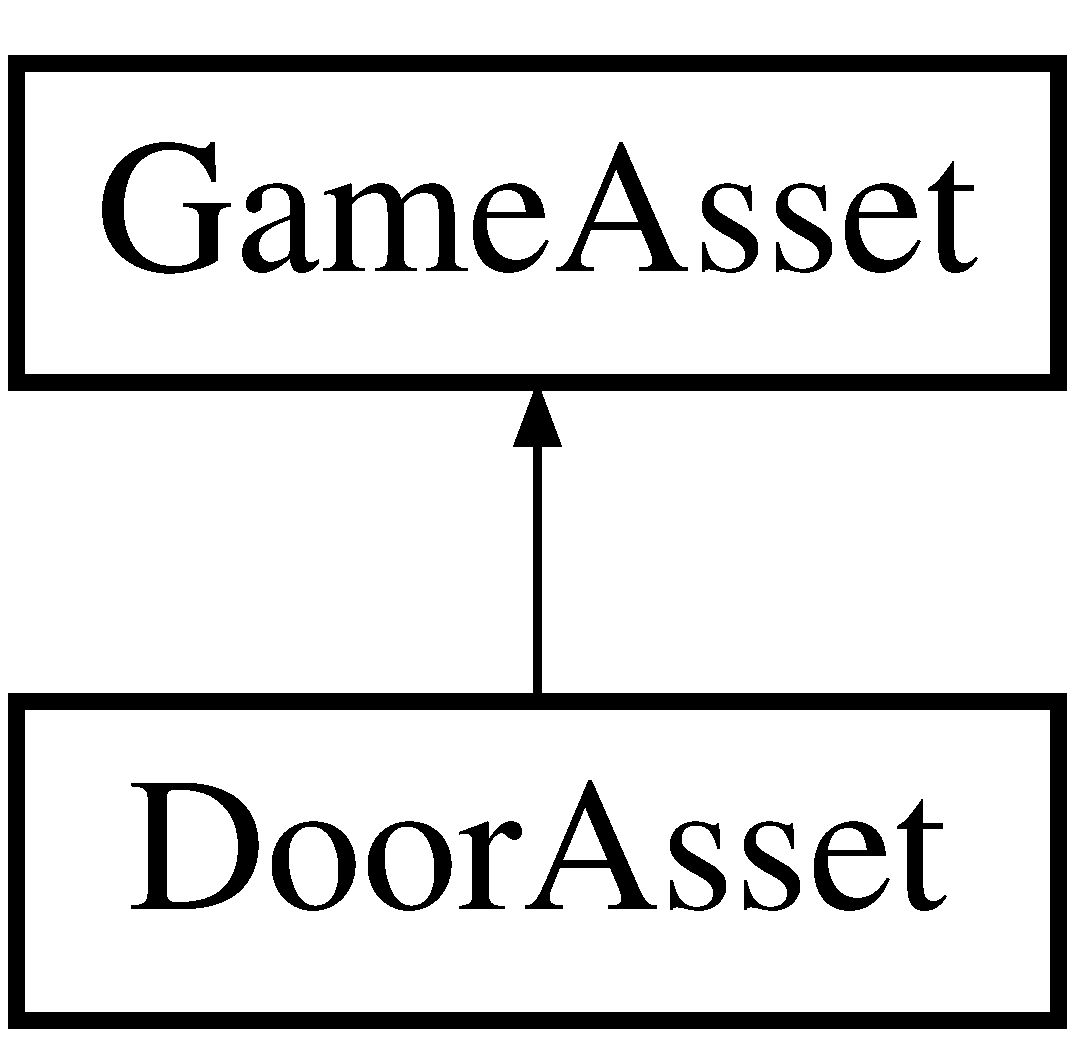
\includegraphics[height=2.000000cm]{classDoorAsset}
\end{center}
\end{figure}
\subsection*{Public Member Functions}
\begin{DoxyCompactItemize}
\item 
virtual void \hyperlink{classDoorAsset_a6b8f73d8bdb9e4e174716ff7231b5fce}{Draw} (G\-Luint program\-I\-D, \hyperlink{classCamera}{Camera} player)
\item 
virtual void \hyperlink{classDoorAsset_a50a91283e458295ddd01530f212b366a}{New\-Position} (vec3)
\item 
virtual bool \hyperlink{classDoorAsset_ae8fc662305af16640ab6e97cfce29360}{Collides} (const shared\-\_\-ptr$<$ \hyperlink{classBounding}{Bounding} $>$ b)
\item 
virtual vec3 \hyperlink{classDoorAsset_ae6f877068ee869b5e9e20eb7d75babba}{Get\-Pos} ()
\item 
virtual std\-::shared\-\_\-ptr$<$ \hyperlink{classBounding}{Bounding} $>$ \hyperlink{classDoorAsset_aacd295e8f653de1465c6febd923f439c}{Get\-Box} ()
\end{DoxyCompactItemize}


\subsection{Detailed Description}
This \hyperlink{classGameAsset}{Game\-Asset} is the door which the player will use to transition between the levels. Its design is extremely similar to the cube, except that it is rectangular instead of cuboid. 

\subsection{Member Function Documentation}
\hypertarget{classDoorAsset_ae8fc662305af16640ab6e97cfce29360}{\index{Door\-Asset@{Door\-Asset}!Collides@{Collides}}
\index{Collides@{Collides}!DoorAsset@{Door\-Asset}}
\subsubsection[{Collides}]{\setlength{\rightskip}{0pt plus 5cm}bool Door\-Asset\-::\-Collides (
\begin{DoxyParamCaption}
\item[{const shared\-\_\-ptr$<$ {\bf Bounding} $>$}]{b}
\end{DoxyParamCaption}
)\hspace{0.3cm}{\ttfamily [virtual]}}}\label{classDoorAsset_ae8fc662305af16640ab6e97cfce29360}
Returns true if two things are colliding 

Implements \hyperlink{classGameAsset}{Game\-Asset}.

\hypertarget{classDoorAsset_a6b8f73d8bdb9e4e174716ff7231b5fce}{\index{Door\-Asset@{Door\-Asset}!Draw@{Draw}}
\index{Draw@{Draw}!DoorAsset@{Door\-Asset}}
\subsubsection[{Draw}]{\setlength{\rightskip}{0pt plus 5cm}void Door\-Asset\-::\-Draw (
\begin{DoxyParamCaption}
\item[{G\-Luint}]{program\-I\-D, }
\item[{{\bf Camera}}]{player}
\end{DoxyParamCaption}
)\hspace{0.3cm}{\ttfamily [virtual]}}}\label{classDoorAsset_a6b8f73d8bdb9e4e174716ff7231b5fce}
Draws the door onto the screen 

Implements \hyperlink{classGameAsset}{Game\-Asset}.

\hypertarget{classDoorAsset_aacd295e8f653de1465c6febd923f439c}{\index{Door\-Asset@{Door\-Asset}!Get\-Box@{Get\-Box}}
\index{Get\-Box@{Get\-Box}!DoorAsset@{Door\-Asset}}
\subsubsection[{Get\-Box}]{\setlength{\rightskip}{0pt plus 5cm}std\-::shared\-\_\-ptr$<$ {\bf Bounding} $>$ Door\-Asset\-::\-Get\-Box (
\begin{DoxyParamCaption}
{}
\end{DoxyParamCaption}
)\hspace{0.3cm}{\ttfamily [virtual]}}}\label{classDoorAsset_aacd295e8f653de1465c6febd923f439c}
Obtains the assets B\-B 

Implements \hyperlink{classGameAsset}{Game\-Asset}.

\hypertarget{classDoorAsset_ae6f877068ee869b5e9e20eb7d75babba}{\index{Door\-Asset@{Door\-Asset}!Get\-Pos@{Get\-Pos}}
\index{Get\-Pos@{Get\-Pos}!DoorAsset@{Door\-Asset}}
\subsubsection[{Get\-Pos}]{\setlength{\rightskip}{0pt plus 5cm}vec3 Door\-Asset\-::\-Get\-Pos (
\begin{DoxyParamCaption}
{}
\end{DoxyParamCaption}
)\hspace{0.3cm}{\ttfamily [virtual]}}}\label{classDoorAsset_ae6f877068ee869b5e9e20eb7d75babba}
Returns the doors position 

Implements \hyperlink{classGameAsset}{Game\-Asset}.

\hypertarget{classDoorAsset_a50a91283e458295ddd01530f212b366a}{\index{Door\-Asset@{Door\-Asset}!New\-Position@{New\-Position}}
\index{New\-Position@{New\-Position}!DoorAsset@{Door\-Asset}}
\subsubsection[{New\-Position}]{\setlength{\rightskip}{0pt plus 5cm}void Door\-Asset\-::\-New\-Position (
\begin{DoxyParamCaption}
\item[{vec3}]{pos}
\end{DoxyParamCaption}
)\hspace{0.3cm}{\ttfamily [virtual]}}}\label{classDoorAsset_a50a91283e458295ddd01530f212b366a}
Sets a new translating position 

The documentation for this class was generated from the following files\-:\begin{DoxyCompactItemize}
\item 
src/Door\-Asset.\-h\item 
src/Door\-Asset.\-cpp\end{DoxyCompactItemize}

\hypertarget{classEvents}{\section{Events Class Reference}
\label{classEvents}\index{Events@{Events}}
}


{\ttfamily \#include $<$events.\-h$>$}

\subsection*{Public Member Functions}
\begin{DoxyCompactItemize}
\item 
bool \hyperlink{classEvents_a07e6042ebb51129e7c7fb02bc8289f9d}{handle\-Events} (S\-D\-L\-\_\-\-Event $\ast$event)
\end{DoxyCompactItemize}


\subsection{Detailed Description}
\hyperlink{classEvents}{Events} is responsible for handling the inputs from the keyboard and the mouse. It also has its own delta time, to help make the game run smoothly. 

\subsection{Member Function Documentation}
\hypertarget{classEvents_a07e6042ebb51129e7c7fb02bc8289f9d}{\index{Events@{Events}!handle\-Events@{handle\-Events}}
\index{handle\-Events@{handle\-Events}!Events@{Events}}
\subsubsection[{handle\-Events}]{\setlength{\rightskip}{0pt plus 5cm}bool Events\-::handle\-Events (
\begin{DoxyParamCaption}
\item[{S\-D\-L\-\_\-\-Event $\ast$}]{event}
\end{DoxyParamCaption}
)}}\label{classEvents_a07e6042ebb51129e7c7fb02bc8289f9d}
Goes through individual key inputs to determine if they have been pressed, and then react accordingly. 

The documentation for this class was generated from the following files\-:\begin{DoxyCompactItemize}
\item 
src/events.\-h\item 
src/events.\-cpp\end{DoxyCompactItemize}

\hypertarget{classGameAsset}{\section{Game\-Asset Class Reference}
\label{classGameAsset}\index{Game\-Asset@{Game\-Asset}}
}


{\ttfamily \#include $<$game\-Asset.\-h$>$}

Inheritance diagram for Game\-Asset\-:\begin{figure}[H]
\begin{center}
\leavevmode
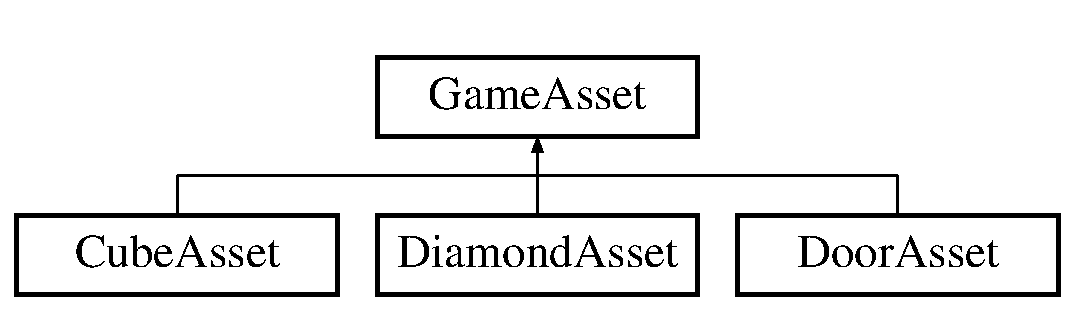
\includegraphics[height=2.000000cm]{classGameAsset}
\end{center}
\end{figure}
\subsection*{Public Member Functions}
\begin{DoxyCompactItemize}
\item 
\hypertarget{classGameAsset_a92268ca0263abe7b9872b77715b50738}{virtual void {\bfseries Draw} (G\-Luint program\-I\-D, \hyperlink{classCamera}{Camera} player)=0}\label{classGameAsset_a92268ca0263abe7b9872b77715b50738}

\item 
\hypertarget{classGameAsset_a2d2ea486dabaf5f437097d5067fddb2e}{virtual void {\bfseries New\-Position} (glm\-::vec3)=0}\label{classGameAsset_a2d2ea486dabaf5f437097d5067fddb2e}

\item 
\hypertarget{classGameAsset_aea9cba492bd511d352743aa2ca997987}{virtual bool {\bfseries Collides} (shared\-\_\-ptr$<$ \hyperlink{classBounding}{Bounding} $>$)=0}\label{classGameAsset_aea9cba492bd511d352743aa2ca997987}

\item 
\hypertarget{classGameAsset_a15c1762c2ece860d861cf03109a06093}{virtual vec3 {\bfseries Get\-Pos} ()=0}\label{classGameAsset_a15c1762c2ece860d861cf03109a06093}

\item 
\hypertarget{classGameAsset_a1b58e9f5e9603a0e9bd014bc466c30bd}{virtual std\-::shared\-\_\-ptr$<$ \hyperlink{classBounding}{Bounding} $>$ {\bfseries Get\-Box} ()=0}\label{classGameAsset_a1b58e9f5e9603a0e9bd014bc466c30bd}

\end{DoxyCompactItemize}


\subsection{Detailed Description}
Creates a standard for the gameassetmanager to create a vector of this types allowing it to store the different cube types, such as diamonds and doors, in a single vector. 

The documentation for this class was generated from the following file\-:\begin{DoxyCompactItemize}
\item 
src/game\-Asset.\-h\end{DoxyCompactItemize}

\hypertarget{classGameAssetManager}{\section{Game\-Asset\-Manager Class Reference}
\label{classGameAssetManager}\index{Game\-Asset\-Manager@{Game\-Asset\-Manager}}
}


{\ttfamily \#include $<$game\-Asset\-Manager.\-h$>$}

\subsection*{Public Member Functions}
\begin{DoxyCompactItemize}
\item 
\hyperlink{classGameAssetManager_a84d0445928649e0d1e0f8e31ee137b17}{Game\-Asset\-Manager} ()
\item 
\hyperlink{classGameAssetManager_a1270bd61ecbcca563f079803e40c9b77}{$\sim$\-Game\-Asset\-Manager} ()
\item 
void \hyperlink{classGameAssetManager_ad3de8ff00d55ba04728b1de8213b2349}{Add\-Asset} (std\-::shared\-\_\-ptr$<$ \hyperlink{classGameAsset}{Game\-Asset} $>$)
\item 
void \hyperlink{classGameAssetManager_a32837132bd70a9a9ed537323c2d3d886}{Draw} ()
\item 
void \hyperlink{classGameAssetManager_ac9dfdde0628476af5b77b60d461041f1}{Move} (int num, glm\-::vec3 pos)
\item 
bool \hyperlink{classGameAssetManager_a79e400319fb874ae0301a8b0e7926737}{Collision} (int n1, const shared\-\_\-ptr$<$ \hyperlink{classBounding}{Bounding} $>$ b)
\item 
void \hyperlink{classGameAssetManager_a9c2f2b3bae3f4752be16e850e9c45136}{Clear} ()
\item 
void \hyperlink{classGameAssetManager_ae7e76a05368ce0887ed72a9ee39329eb}{Intelligence} (int cubes, int diamonds)
\item 
void \hyperlink{classGameAssetManager_a2c87c005095eadb1669428dfe3a16423}{Remove} (int num)
\item 
int \hyperlink{classGameAssetManager_ae0e0f79e6dbe422ce5d3c4fd5e20d032}{Size} ()
\end{DoxyCompactItemize}


\subsection{Detailed Description}
\hyperlink{classGameAssetManager}{Game\-Asset\-Manager} is a container for Game\-Assets. It also provides utility functions to to create a simple Open\-G\-L program that can be used to draw a simple \hyperlink{classGameAsset}{Game\-Asset}. 

\subsection{Constructor \& Destructor Documentation}
\hypertarget{classGameAssetManager_a84d0445928649e0d1e0f8e31ee137b17}{\index{Game\-Asset\-Manager@{Game\-Asset\-Manager}!Game\-Asset\-Manager@{Game\-Asset\-Manager}}
\index{Game\-Asset\-Manager@{Game\-Asset\-Manager}!GameAssetManager@{Game\-Asset\-Manager}}
\subsubsection[{Game\-Asset\-Manager}]{\setlength{\rightskip}{0pt plus 5cm}Game\-Asset\-Manager\-::\-Game\-Asset\-Manager (
\begin{DoxyParamCaption}
{}
\end{DoxyParamCaption}
)}}\label{classGameAssetManager_a84d0445928649e0d1e0f8e31ee137b17}
Creates a \hyperlink{classGameAssetManager}{Game\-Asset\-Manager} to load the correct shaders based on the Application\-Mode. \hypertarget{classGameAssetManager_a1270bd61ecbcca563f079803e40c9b77}{\index{Game\-Asset\-Manager@{Game\-Asset\-Manager}!$\sim$\-Game\-Asset\-Manager@{$\sim$\-Game\-Asset\-Manager}}
\index{$\sim$\-Game\-Asset\-Manager@{$\sim$\-Game\-Asset\-Manager}!GameAssetManager@{Game\-Asset\-Manager}}
\subsubsection[{$\sim$\-Game\-Asset\-Manager}]{\setlength{\rightskip}{0pt plus 5cm}Game\-Asset\-Manager\-::$\sim$\-Game\-Asset\-Manager (
\begin{DoxyParamCaption}
{}
\end{DoxyParamCaption}
)}}\label{classGameAssetManager_a1270bd61ecbcca563f079803e40c9b77}
Deletes the program\-I\-D, the pointer to the shaders 

\subsection{Member Function Documentation}
\hypertarget{classGameAssetManager_ad3de8ff00d55ba04728b1de8213b2349}{\index{Game\-Asset\-Manager@{Game\-Asset\-Manager}!Add\-Asset@{Add\-Asset}}
\index{Add\-Asset@{Add\-Asset}!GameAssetManager@{Game\-Asset\-Manager}}
\subsubsection[{Add\-Asset}]{\setlength{\rightskip}{0pt plus 5cm}void Game\-Asset\-Manager\-::\-Add\-Asset (
\begin{DoxyParamCaption}
\item[{std\-::shared\-\_\-ptr$<$ {\bf Game\-Asset} $>$}]{the\-\_\-asset}
\end{DoxyParamCaption}
)}}\label{classGameAssetManager_ad3de8ff00d55ba04728b1de8213b2349}
Adds a \hyperlink{classGameAsset}{Game\-Asset} to the scene graph. \hypertarget{classGameAssetManager_a9c2f2b3bae3f4752be16e850e9c45136}{\index{Game\-Asset\-Manager@{Game\-Asset\-Manager}!Clear@{Clear}}
\index{Clear@{Clear}!GameAssetManager@{Game\-Asset\-Manager}}
\subsubsection[{Clear}]{\setlength{\rightskip}{0pt plus 5cm}void Game\-Asset\-Manager\-::\-Clear (
\begin{DoxyParamCaption}
{}
\end{DoxyParamCaption}
)}}\label{classGameAssetManager_a9c2f2b3bae3f4752be16e850e9c45136}
Empties the draw vector, allowing for the next levels cubes to load \hypertarget{classGameAssetManager_a79e400319fb874ae0301a8b0e7926737}{\index{Game\-Asset\-Manager@{Game\-Asset\-Manager}!Collision@{Collision}}
\index{Collision@{Collision}!GameAssetManager@{Game\-Asset\-Manager}}
\subsubsection[{Collision}]{\setlength{\rightskip}{0pt plus 5cm}bool Game\-Asset\-Manager\-::\-Collision (
\begin{DoxyParamCaption}
\item[{int}]{n1, }
\item[{const shared\-\_\-ptr$<$ {\bf Bounding} $>$}]{b}
\end{DoxyParamCaption}
)}}\label{classGameAssetManager_a79e400319fb874ae0301a8b0e7926737}
Checks if two objects are colliding \hypertarget{classGameAssetManager_a32837132bd70a9a9ed537323c2d3d886}{\index{Game\-Asset\-Manager@{Game\-Asset\-Manager}!Draw@{Draw}}
\index{Draw@{Draw}!GameAssetManager@{Game\-Asset\-Manager}}
\subsubsection[{Draw}]{\setlength{\rightskip}{0pt plus 5cm}void Game\-Asset\-Manager\-::\-Draw (
\begin{DoxyParamCaption}
{}
\end{DoxyParamCaption}
)}}\label{classGameAssetManager_a32837132bd70a9a9ed537323c2d3d886}
Draws each \hyperlink{classGameAsset}{Game\-Asset} in the scene graph. \hypertarget{classGameAssetManager_ae7e76a05368ce0887ed72a9ee39329eb}{\index{Game\-Asset\-Manager@{Game\-Asset\-Manager}!Intelligence@{Intelligence}}
\index{Intelligence@{Intelligence}!GameAssetManager@{Game\-Asset\-Manager}}
\subsubsection[{Intelligence}]{\setlength{\rightskip}{0pt plus 5cm}void Game\-Asset\-Manager\-::\-Intelligence (
\begin{DoxyParamCaption}
\item[{int}]{cubes, }
\item[{int}]{diamonds}
\end{DoxyParamCaption}
)}}\label{classGameAssetManager_ae7e76a05368ce0887ed72a9ee39329eb}
Follows an algorithm which makes the diamond shy away from the player, causing it to retreat in the opposite direction of the player. \hypertarget{classGameAssetManager_ac9dfdde0628476af5b77b60d461041f1}{\index{Game\-Asset\-Manager@{Game\-Asset\-Manager}!Move@{Move}}
\index{Move@{Move}!GameAssetManager@{Game\-Asset\-Manager}}
\subsubsection[{Move}]{\setlength{\rightskip}{0pt plus 5cm}void Game\-Asset\-Manager\-::\-Move (
\begin{DoxyParamCaption}
\item[{int}]{num, }
\item[{glm\-::vec3}]{pos}
\end{DoxyParamCaption}
)}}\label{classGameAssetManager_ac9dfdde0628476af5b77b60d461041f1}
Changes the vec3 of an asset, transitioning it \hypertarget{classGameAssetManager_a2c87c005095eadb1669428dfe3a16423}{\index{Game\-Asset\-Manager@{Game\-Asset\-Manager}!Remove@{Remove}}
\index{Remove@{Remove}!GameAssetManager@{Game\-Asset\-Manager}}
\subsubsection[{Remove}]{\setlength{\rightskip}{0pt plus 5cm}void Game\-Asset\-Manager\-::\-Remove (
\begin{DoxyParamCaption}
\item[{int}]{num}
\end{DoxyParamCaption}
)}}\label{classGameAssetManager_a2c87c005095eadb1669428dfe3a16423}
Removes an asset from the list \hypertarget{classGameAssetManager_ae0e0f79e6dbe422ce5d3c4fd5e20d032}{\index{Game\-Asset\-Manager@{Game\-Asset\-Manager}!Size@{Size}}
\index{Size@{Size}!GameAssetManager@{Game\-Asset\-Manager}}
\subsubsection[{Size}]{\setlength{\rightskip}{0pt plus 5cm}int Game\-Asset\-Manager\-::\-Size (
\begin{DoxyParamCaption}
{}
\end{DoxyParamCaption}
)}}\label{classGameAssetManager_ae0e0f79e6dbe422ce5d3c4fd5e20d032}
Returns the size of the vector 

The documentation for this class was generated from the following files\-:\begin{DoxyCompactItemize}
\item 
src/game\-Asset\-Manager.\-h\item 
src/game\-Asset\-Manager.\-cpp\end{DoxyCompactItemize}

\hypertarget{classLevel}{\section{Level Class Reference}
\label{classLevel}\index{Level@{Level}}
}


{\ttfamily \#include $<$level.\-h$>$}

\subsection*{Public Member Functions}
\begin{DoxyCompactItemize}
\item 
bool \hyperlink{classLevel_a09cffeaf0d6f4a583f5a83f1a07cd0ad}{run\-Level} (int lvl, S\-D\-L\-\_\-\-Window $\ast$window)
\item 
int \hyperlink{classLevel_a427e559e6b7dab9867c76cef6eab4185}{block\-Positions} ()
\item 
bool \hyperlink{classLevel_a0d16d2fbefe76a3b5e5bcb2ad4e6a6c2}{fill\-Vector} (int lvl)
\item 
bool \hyperlink{classLevel_a8651318bbd27c04e5105e4bc4593173a}{collision\-Detection} (int lvl)
\item 
void \hyperlink{classLevel_a24eeee2748d12fd613ad3fb86b1557d9}{sky} ()
\end{DoxyCompactItemize}


\subsection{Detailed Description}
This class runs the inner loop for all the individual levels, which means receiving inputs, checking collision, drawing the cubes. It is also responsible reading cube positions, from the .json files and then passing them to the gameassetmanager to manipulate them. 

\subsection{Member Function Documentation}
\hypertarget{classLevel_a427e559e6b7dab9867c76cef6eab4185}{\index{Level@{Level}!block\-Positions@{block\-Positions}}
\index{block\-Positions@{block\-Positions}!Level@{Level}}
\subsubsection[{block\-Positions}]{\setlength{\rightskip}{0pt plus 5cm}int Level\-::block\-Positions (
\begin{DoxyParamCaption}
{}
\end{DoxyParamCaption}
)}}\label{classLevel_a427e559e6b7dab9867c76cef6eab4185}
Adds assets to the gameassetmanager, then translates them by vec3 positions from the cubepositons vector \hypertarget{classLevel_a8651318bbd27c04e5105e4bc4593173a}{\index{Level@{Level}!collision\-Detection@{collision\-Detection}}
\index{collision\-Detection@{collision\-Detection}!Level@{Level}}
\subsubsection[{collision\-Detection}]{\setlength{\rightskip}{0pt plus 5cm}bool Level\-::collision\-Detection (
\begin{DoxyParamCaption}
\item[{int}]{lvl}
\end{DoxyParamCaption}
)}}\label{classLevel_a8651318bbd27c04e5105e4bc4593173a}
Goes through loops, checking if the player collides with cubes, diamonds and the door. The return value determines what the boolean gravity is (True or False). \begin{DoxyRefDesc}{Bug}
\item[\hyperlink{bug__bug000001}{Bug}]can collide within the cube. \end{DoxyRefDesc}
\hypertarget{classLevel_a0d16d2fbefe76a3b5e5bcb2ad4e6a6c2}{\index{Level@{Level}!fill\-Vector@{fill\-Vector}}
\index{fill\-Vector@{fill\-Vector}!Level@{Level}}
\subsubsection[{fill\-Vector}]{\setlength{\rightskip}{0pt plus 5cm}bool Level\-::fill\-Vector (
\begin{DoxyParamCaption}
\item[{int}]{lvl}
\end{DoxyParamCaption}
)}}\label{classLevel_a0d16d2fbefe76a3b5e5bcb2ad4e6a6c2}
Reads in x, y and z positions from individual .json positions -\/ depending on int level \hypertarget{classLevel_a09cffeaf0d6f4a583f5a83f1a07cd0ad}{\index{Level@{Level}!run\-Level@{run\-Level}}
\index{run\-Level@{run\-Level}!Level@{Level}}
\subsubsection[{run\-Level}]{\setlength{\rightskip}{0pt plus 5cm}bool Level\-::run\-Level (
\begin{DoxyParamCaption}
\item[{int}]{lvl, }
\item[{S\-D\-L\-\_\-\-Window $\ast$}]{window}
\end{DoxyParamCaption}
)}}\label{classLevel_a09cffeaf0d6f4a583f5a83f1a07cd0ad}
This method runs the second loop within the game (The level loop). It begins by filling a vector with cube positions, before then passing them into individual game assets. Finally it begins the loop, where it receives inputs, updates then draws. \hypertarget{classLevel_a24eeee2748d12fd613ad3fb86b1557d9}{\index{Level@{Level}!sky@{sky}}
\index{sky@{sky}!Level@{Level}}
\subsubsection[{sky}]{\setlength{\rightskip}{0pt plus 5cm}void Level\-::sky (
\begin{DoxyParamCaption}
{}
\end{DoxyParamCaption}
)}}\label{classLevel_a24eeee2748d12fd613ad3fb86b1557d9}
Follows some small rules to change the background frame colour from night to day! Uses r g b variables 

The documentation for this class was generated from the following files\-:\begin{DoxyCompactItemize}
\item 
src/level.\-h\item 
src/level.\-cpp\end{DoxyCompactItemize}

%--- End generated contents ---

% Index
\newpage
\phantomsection
\addcontentsline{toc}{chapter}{Index}
\printindex

\end{document}
